\chapter{Extension: Higher-Order Modulations}\label{sec:extensions}

The core of this thesis (Chapter~\ref{sec:experiments}) answers hypotheses H1--H5 on the canonical setup. This chapter contains one scoped extension: whether the canonical BPSK conclusions generalize to complex constellations. Two studies are reported. The first evaluates QPSK and 16-QAM under the I/Q-splitting formulation, exposing a structural BER floor for multi-level constellations; the second removes that floor by reformulating the relay as a joint $N$-class classifier over the full 2D constellation ($N=16$ for 16-QAM). These analyses adopt the channel configurations under which they were conducted (AWGN and Rayleigh for the first study, AWGN for the second); MIMO, 16-PSK, CSI injection, and end-to-end learning remain future work. The separate question of how classical and learned relays behave when the \emph{channel itself} is unknown or mismatched, a more substantial investigation, forms the dedicated contribution of Chapter~\ref{sec:unknown-channels}.

\section{Higher-Order Modulation Scalability (Constellation-Aware Training)}\label{sec:higher-order-modulation-scalability-constellation-aware-training}

\textbf{Goal:} Evaluate the generalizability of BPSK-trained relays to complex constellations and resolve the multi-level amplitude bottleneck.

\textbf{Trials:} - \textbf{Topology:} SISO - \textbf{Modulation scheme:} QPSK, 16-QAM - \textbf{Channel:} AWGN, Rayleigh - \textbf{Equalizers:} None - \textbf{NN architecture:} Supervised (MLP, Hybrid), Generative (VAE, CGAN), Sequence (Transformer, Mamba S6, Mamba-2 SSD) - \textbf{NN output activation (swept):} tanh, linear, clipped tanh (hardtanh), scaled tanh, scaled sigmoid (ReLU hidden throughout) - \textbf{Special case:} Constellation Aware training

\textbf{Conclusion:} QPSK performance mirrors BPSK perfectly due to I/Q independence. On 16-QAM, standard tanh compression causes a severe, irreducible BER floor (\textasciitilde0.22 at 16 dB). Replacing tanh with constellation-aware bounded activations (hardtanh, scaled tanh) bounded to the precise signal amplitude (\(3/\sqrt{10}\)) and retraining eliminates this floor. Sequence models benefit most, reducing their BER floor by 5x, though a gap to classical DF persists due to per-axis error accumulation, the limitation removed by the 2D classification study below.

\subsection{Results Tables}\label{sec:results-tables-3}

\begin{longtable}[]{@{}
  >{\raggedright\arraybackslash}p{(\linewidth - 14\tabcolsep) * \real{0.1250}}
  >{\raggedright\arraybackslash}p{(\linewidth - 14\tabcolsep) * \real{0.1250}}
  >{\raggedright\arraybackslash}p{(\linewidth - 14\tabcolsep) * \real{0.1250}}
  >{\raggedright\arraybackslash}p{(\linewidth - 14\tabcolsep) * \real{0.1250}}
  >{\raggedright\arraybackslash}p{(\linewidth - 14\tabcolsep) * \real{0.1250}}
  >{\raggedright\arraybackslash}p{(\linewidth - 14\tabcolsep) * \real{0.1250}}
  >{\raggedright\arraybackslash}p{(\linewidth - 14\tabcolsep) * \real{0.1250}}
  >{\raggedright\arraybackslash}p{(\linewidth - 14\tabcolsep) * \real{0.1250}}@{}}
\caption{BER comparison across modulations at selected SNR points (AWGN channel). All nine relay strategies.}\label{tbl:table14}\tabularnewline
\toprule\noalign{}
\begin{minipage}[b]{\linewidth}\raggedright
Relay
\end{minipage} & \begin{minipage}[b]{\linewidth}\raggedright
BPSK 0 dB
\end{minipage} & \begin{minipage}[b]{\linewidth}\raggedright
BPSK 10 dB
\end{minipage} & \begin{minipage}[b]{\linewidth}\raggedright
QPSK 0 dB
\end{minipage} & \begin{minipage}[b]{\linewidth}\raggedright
QPSK 10 dB
\end{minipage} & \begin{minipage}[b]{\linewidth}\raggedright
16-QAM 0 dB
\end{minipage} & \begin{minipage}[b]{\linewidth}\raggedright
16-QAM 10 dB
\end{minipage} & \begin{minipage}[b]{\linewidth}\raggedright
16-QAM 16 dB
\end{minipage} \\
\midrule\noalign{}
\endfirsthead
\toprule\noalign{}
\begin{minipage}[b]{\linewidth}\raggedright
Relay
\end{minipage} & \begin{minipage}[b]{\linewidth}\raggedright
BPSK 0 dB
\end{minipage} & \begin{minipage}[b]{\linewidth}\raggedright
BPSK 10 dB
\end{minipage} & \begin{minipage}[b]{\linewidth}\raggedright
QPSK 0 dB
\end{minipage} & \begin{minipage}[b]{\linewidth}\raggedright
QPSK 10 dB
\end{minipage} & \begin{minipage}[b]{\linewidth}\raggedright
16-QAM 0 dB
\end{minipage} & \begin{minipage}[b]{\linewidth}\raggedright
16-QAM 10 dB
\end{minipage} & \begin{minipage}[b]{\linewidth}\raggedright
16-QAM 16 dB
\end{minipage} \\
\midrule\noalign{}
\endhead
\bottomrule\noalign{}
\endlastfoot
AF & 0.2813 & 0.0141 & 0.2794 & 0.0142 & 0.3778 & 0.1244 & 0.0180 \\
DF & 0.2651 & 0.0015 & 0.2644 & 0.0016 & 0.3811 & 0.1076 & 0.0038 \\
MLP (169p) & 0.2589 & 0.0021 & 0.2563 & 0.0025 & 0.3907 & 0.2180 & 0.2180 \\
Hybrid & 0.2573 & 0.0015 & 0.2644 & 0.0016 & 0.4000 & 0.2711 & 0.2512 \\
VAE & 0.2611 & 0.0021 & 0.2597 & 0.0036 & 0.3945 & 0.2391 & 0.2231 \\
CGAN (WGAN-GP) & 0.2633 & 0.0017 & 0.2621 & 0.0018 & 0.3976 & 0.2588 & 0.2486 \\
trans-\\former & 0.2593 & 0.0024 & 0.2576 & 0.0036 & 0.3897 & 0.2042 & 0.1827 \\
Mamba S6 & 0.2585 & 0.0021 & 0.2560 & 0.0028 & 0.3894 & 0.2016 & 0.1935 \\
Mamba2 (SSD) & 0.2593 & 0.0023 & 0.2566 & 0.0034 & 0.3903 & 0.2032 & 0.1890 \\
\end{longtable}

Table \ref{tbl:table15} shows the BER at 16 dB for all relays across the three activation variants and both channel types.

\begin{longtable}[]{@{}
  >{\raggedright\arraybackslash}p{(\linewidth - 12\tabcolsep) * \real{0.1429}}
  >{\raggedright\arraybackslash}p{(\linewidth - 12\tabcolsep) * \real{0.1429}}
  >{\raggedright\arraybackslash}p{(\linewidth - 12\tabcolsep) * \real{0.1429}}
  >{\raggedright\arraybackslash}p{(\linewidth - 12\tabcolsep) * \real{0.1429}}
  >{\raggedright\arraybackslash}p{(\linewidth - 12\tabcolsep) * \real{0.1429}}
  >{\raggedright\arraybackslash}p{(\linewidth - 12\tabcolsep) * \real{0.1429}}
  >{\raggedright\arraybackslash}p{(\linewidth - 12\tabcolsep) * \real{0.1429}}@{}}
\caption{BER at 16 dB for all relay variants across activation functions and modulations (AWGN and Rayleigh).}\label{tbl:table15}\tabularnewline
\toprule\noalign{}
\begin{minipage}[b]{\linewidth}\raggedright
Relay
\end{minipage} & \begin{minipage}[b]{\linewidth}\raggedright
tanh (BPSK)
\end{minipage} & \begin{minipage}[b]{\linewidth}\raggedright
linear (QAM16)
\end{minipage} & \begin{minipage}[b]{\linewidth}\raggedright
hardtanh (QAM16)
\end{minipage} & \begin{minipage}[b]{\linewidth}\raggedright
tanh (BPSK)
\end{minipage} & \begin{minipage}[b]{\linewidth}\raggedright
linear (QAM16)
\end{minipage} & \begin{minipage}[b]{\linewidth}\raggedright
hardtanh (QAM16)
\end{minipage} \\
\midrule\noalign{}
\endfirsthead
\toprule\noalign{}
\begin{minipage}[b]{\linewidth}\raggedright
Relay
\end{minipage} & \begin{minipage}[b]{\linewidth}\raggedright
tanh (BPSK)
\end{minipage} & \begin{minipage}[b]{\linewidth}\raggedright
linear (QAM16)
\end{minipage} & \begin{minipage}[b]{\linewidth}\raggedright
hardtanh (QAM16)
\end{minipage} & \begin{minipage}[b]{\linewidth}\raggedright
tanh (BPSK)
\end{minipage} & \begin{minipage}[b]{\linewidth}\raggedright
linear (QAM16)
\end{minipage} & \begin{minipage}[b]{\linewidth}\raggedright
hardtanh (QAM16)
\end{minipage} \\
\midrule\noalign{}
\endhead
\bottomrule\noalign{}
\endlastfoot
& \textbf{AWGN} & & & \textbf{Rayleigh} & & \\
MLP & 0.2202 & 0.0721 & \textbf{0.0630} & 0.2375 & 0.1279 & \textbf{0.1247} \\
Hybrid & 0.2512 & 0.2512 & 0.2512 & 0.2723 & 0.2723 & 0.2723 \\
VAE & 0.2231 & 0.1111 & \textbf{0.1059} & 0.2462 & 0.1575 & \textbf{0.1573} \\
CGAN & 0.2482 & 0.0973 & \textbf{0.0863} & 0.2666 & 0.1432 & \textbf{0.1383} \\
trans-\\former & 0.2111 & \textbf{0.0453} & 0.0505 & 0.2305 & \textbf{0.1159} & 0.1194 \\
Mamba S6 & 0.2131 & 0.0422 & \textbf{0.0396} & 0.2333 & 0.1129 & \textbf{0.1108} \\
Mamba2\\(ssd) & 0.2065 & 0.0471 & \textbf{0.0441} & 0.2273 & 0.1157 & \textbf{0.1145} \\
AF & 0.0180 &: &: & 0.1009 &: &: \\
DF & 0.0038 &: &: & 0.0828 &: &: \\
\end{longtable}


\subsection{Results Figures}\label{sec:results-figures-4}

\begin{figure}[H]
\centering
\centering
\pandocbounded{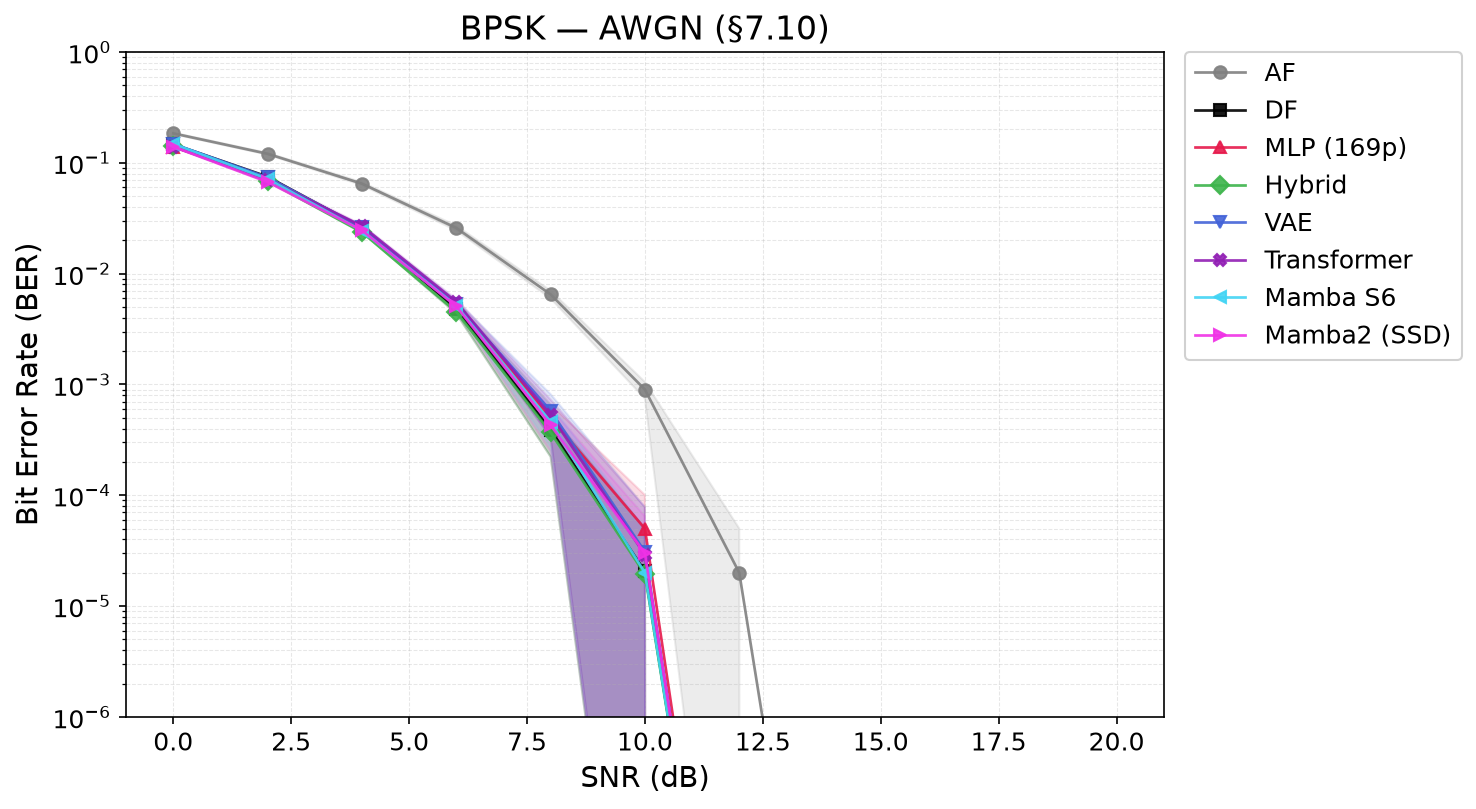
\includegraphics[width=\linewidth,height=0.8\textheight,keepaspectratio]{results/modulation/bpsk_awgn_ci.png}}
\caption{BPSK on AWGN: all relay strategies with 95\% CI (baseline for modulation comparison).}\label{fig:fig21}
\end{figure}

\begin{figure}[H]
\centering
\centering
\pandocbounded{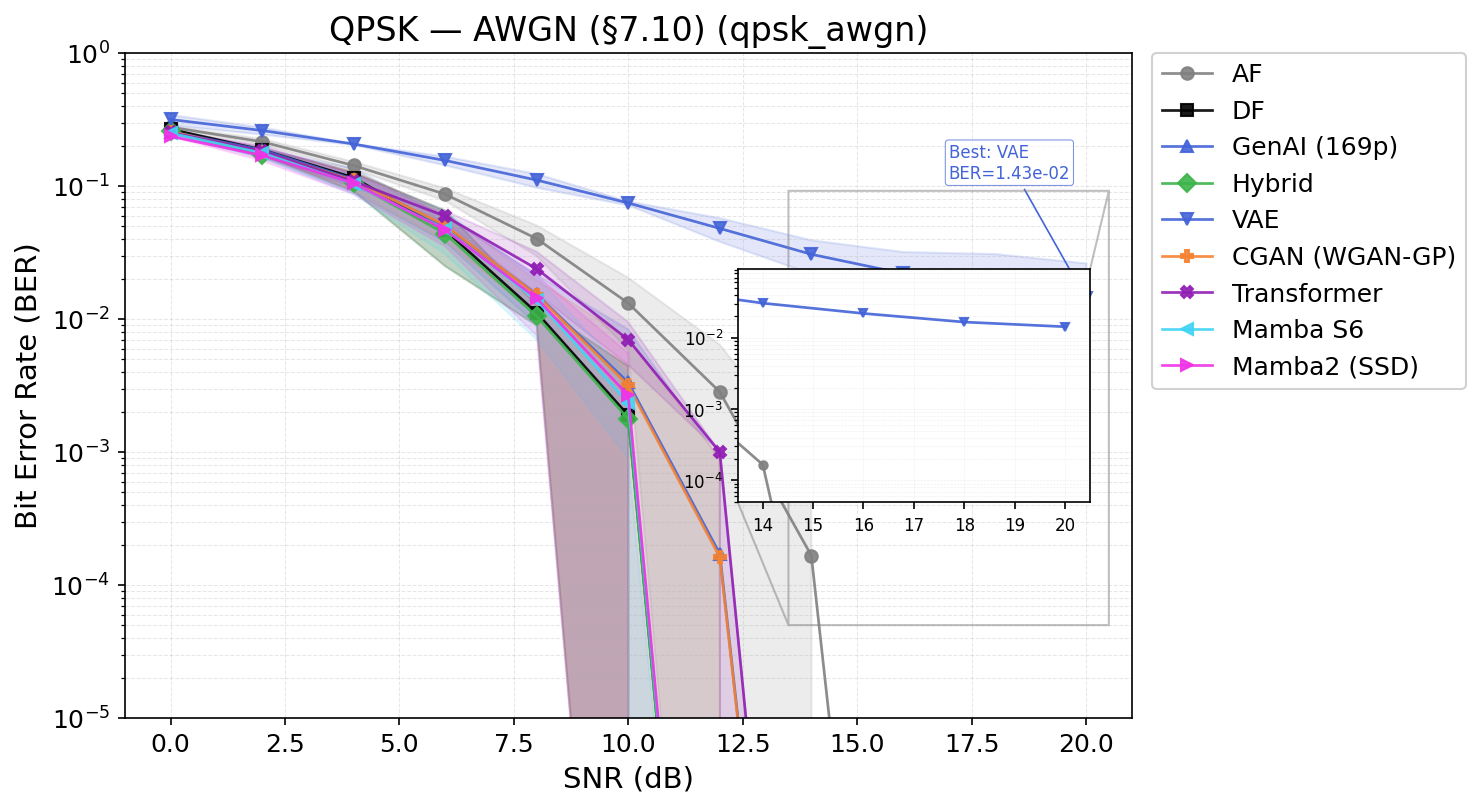
\includegraphics[width=\linewidth,height=\textheight,keepaspectratio]{results/modulation/qpsk_awgn_ci.png}}
\caption{QPSK on AWGN: BER curves closely match the BPSK baseline (\ref{fig:fig21}), confirming I/Q splitting validity.}\label{fig:fig23}
\end{figure}

\begin{figure}[H]
\centering
\centering
\pandocbounded{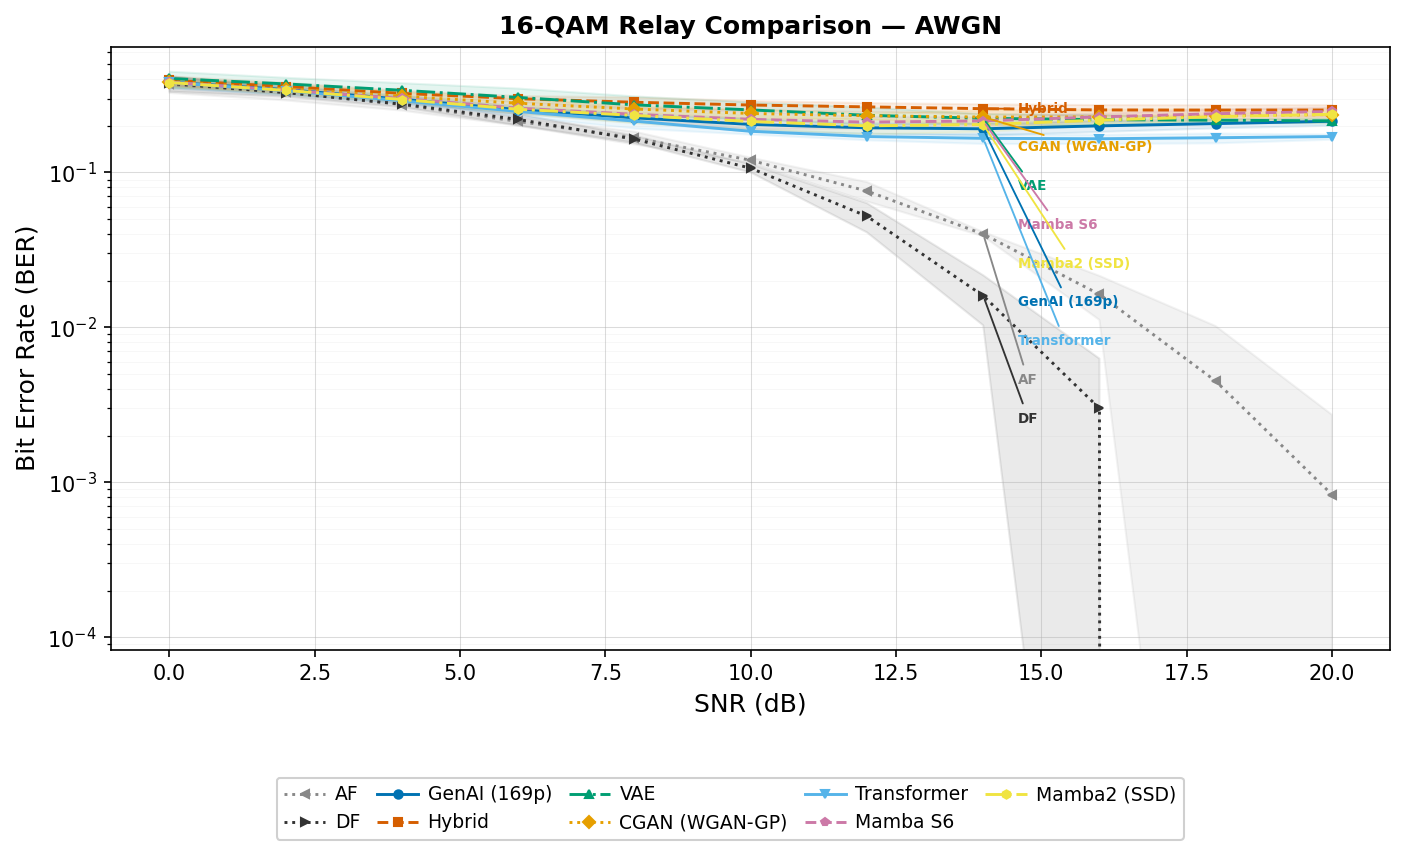
\includegraphics[width=\linewidth,height=\textheight,keepaspectratio]{results/modulation/qam16__awgn_ci.png}}
\caption{16-QAM on AWGN: AI relays hit a BER floor near 0.22 at medium-high SNR due to \(\tanh\) compression of multi-level signals; AF outperforms DF at low SNR.}\label{fig:fig25}
\end{figure}

\begin{figure}[b]
\centering
\centering
\pandocbounded{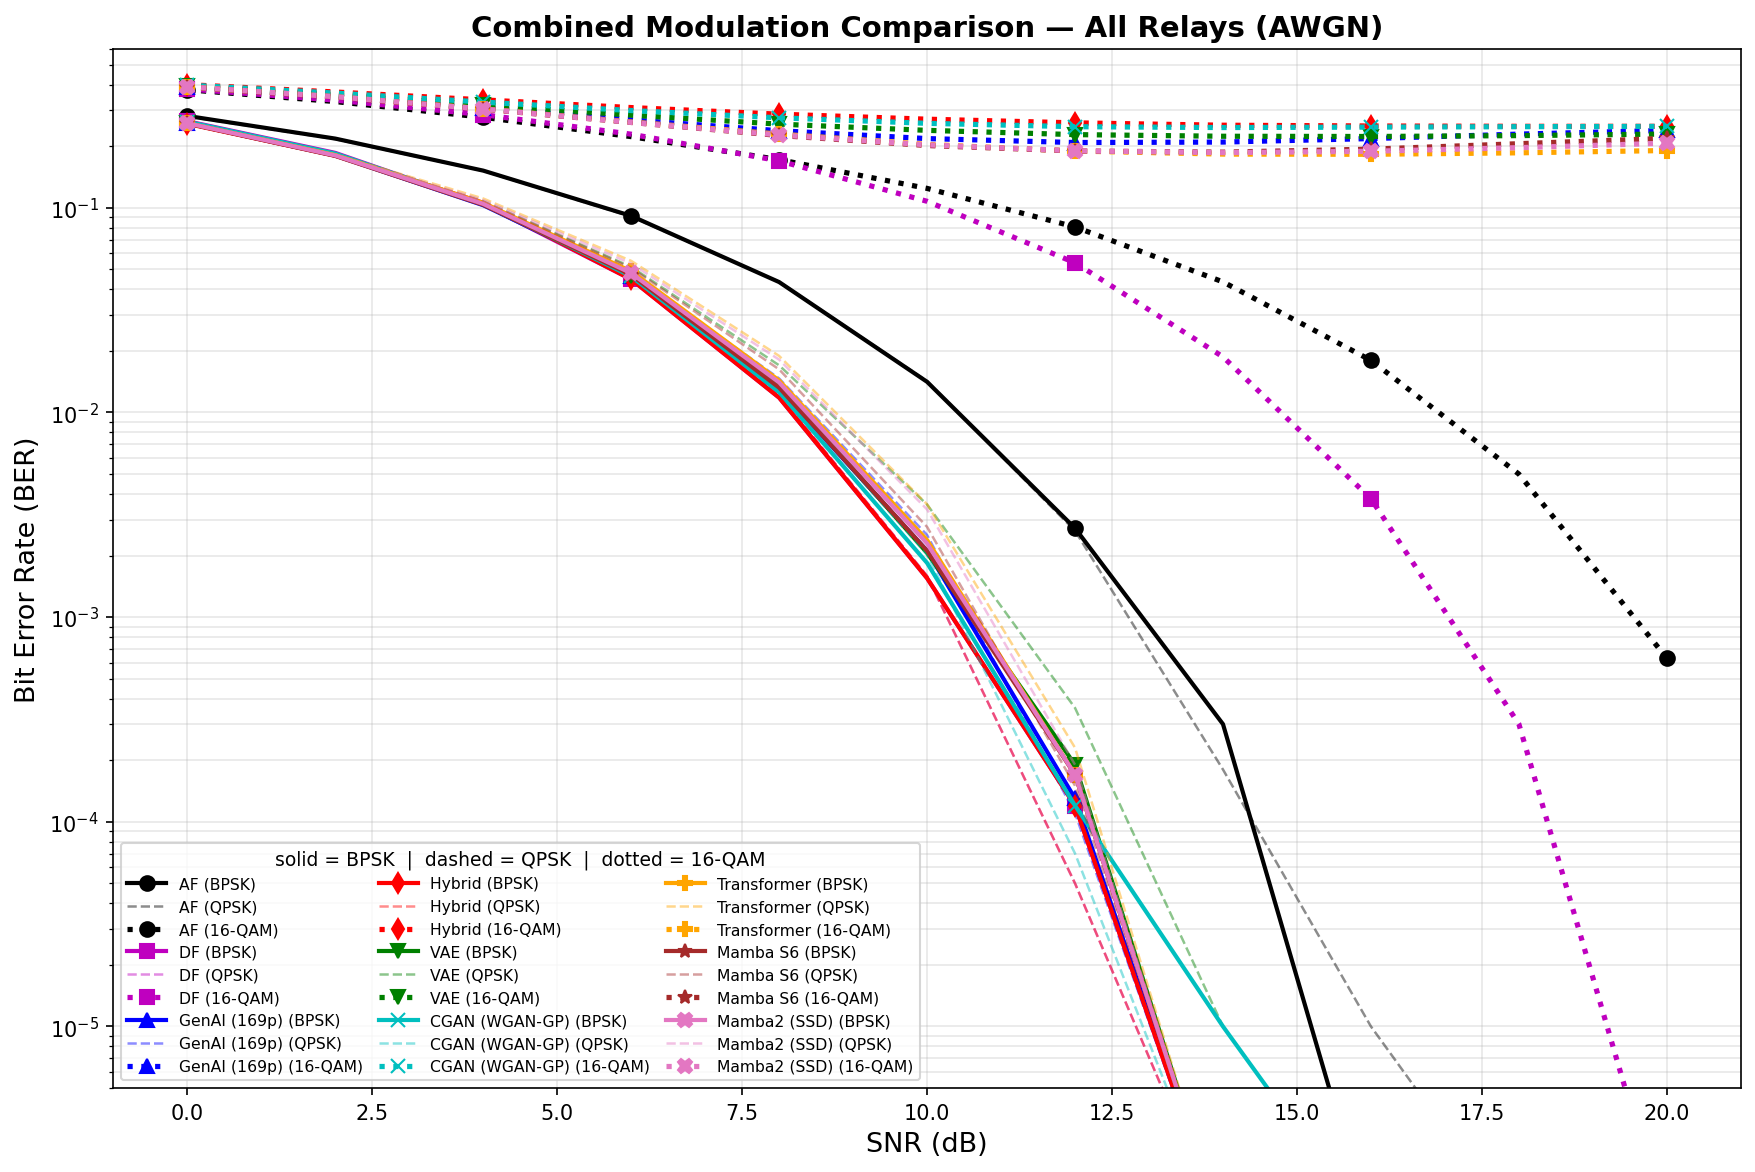
\includegraphics[width=\linewidth,height=\textheight,keepaspectratio]{results/modulation/combined_modulation_awgn.png}}
\caption{Combined modulation comparison (AWGN): all nine relays across BPSK (solid), QPSK (dashed, overlapping BPSK), and 16-QAM (dotted). The BPSK/QPSK overlap confirms I/Q splitting equivalence. The 16-QAM dotted curves reveal the AI relay BER floor: all AI relays plateau near 0.18--0.25 while DF and AF continue decreasing.}\label{fig:fig27}
\end{figure}

% \begin{figure}[H]
% \centering
% \centering
% \pandocbounded{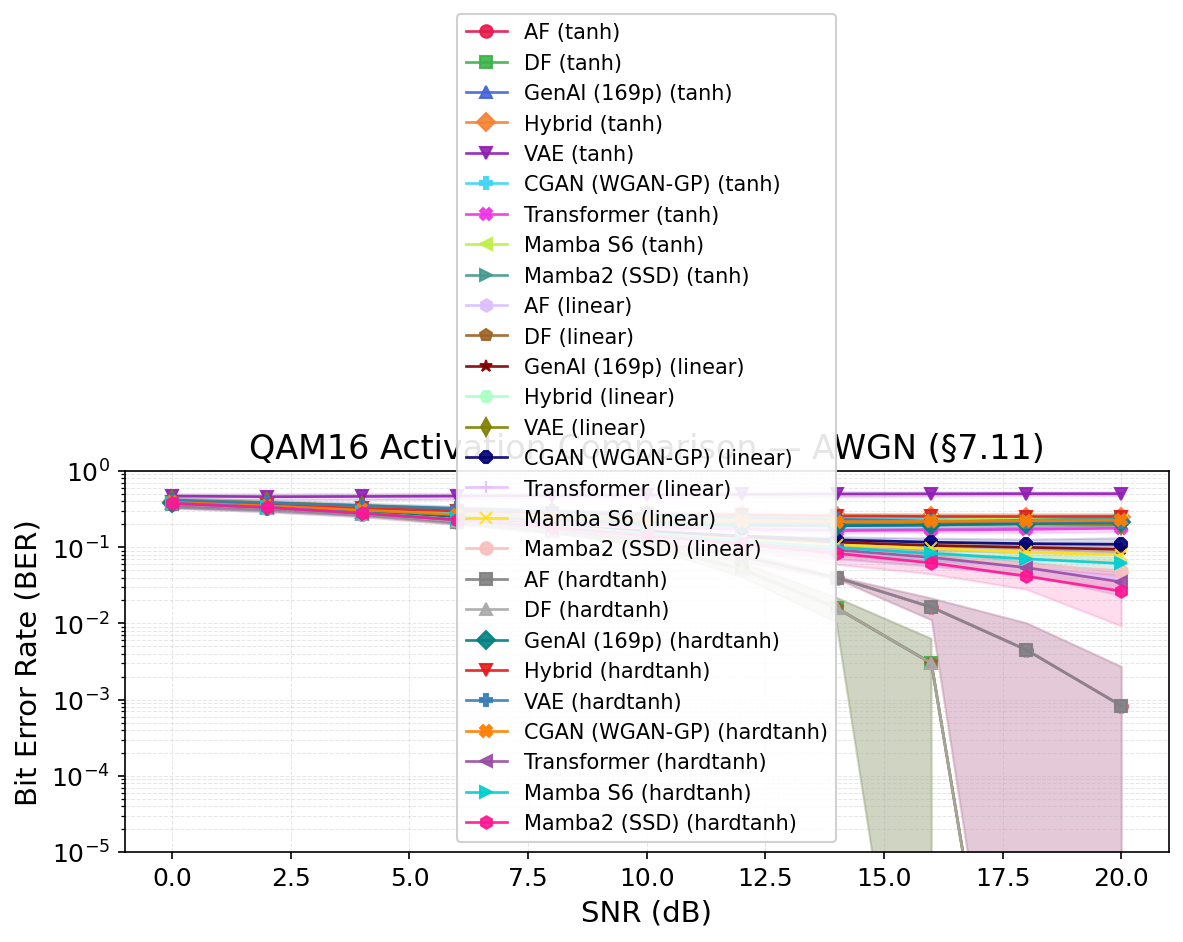
\includegraphics[width=\linewidth,height=\textheight,keepaspectratio]{results/qam16_activation/qam16_activation_awgn.png}}
% \caption{16-QAM activation experiment (AWGN): dashed lines = tanh/BPSK baseline, solid = linear/QAM16, dotted = hardtanh/QAM16. Replacing tanh and retraining on QAM16 eliminates the BER floor for all AI relays except Hybrid. Sequence models (Transformer, Mamba S6, Mamba-2) benefit most, narrowing the gap to DF from \textasciitilde56x to \textasciitilde10x.}\label{fig:fig28}
% \end{figure}


\begin{figure}[H]
    \centering
    
\includegraphics[width=1\linewidth]{results//qam16_activation/qam16_activation_awgn.png}
    \caption{16-QAM activation experiment (AWGN): dashed lines = tanh/BPSK baseline, solid = linear/QAM16, dotted = hardtanh/QAM16. Replacing tanh and retraining on QAM16 eliminates the BER floor for all AI relays except Hybrid. Sequence models (Transformer, Mamba S6, Mamba-2) benefit most, narrowing the gap to DF from \textasciitilde56x to \textasciitilde10x.}
    \label{fig:fig28}
\end{figure}

\begin{figure}[H]

\centering
\pandocbounded{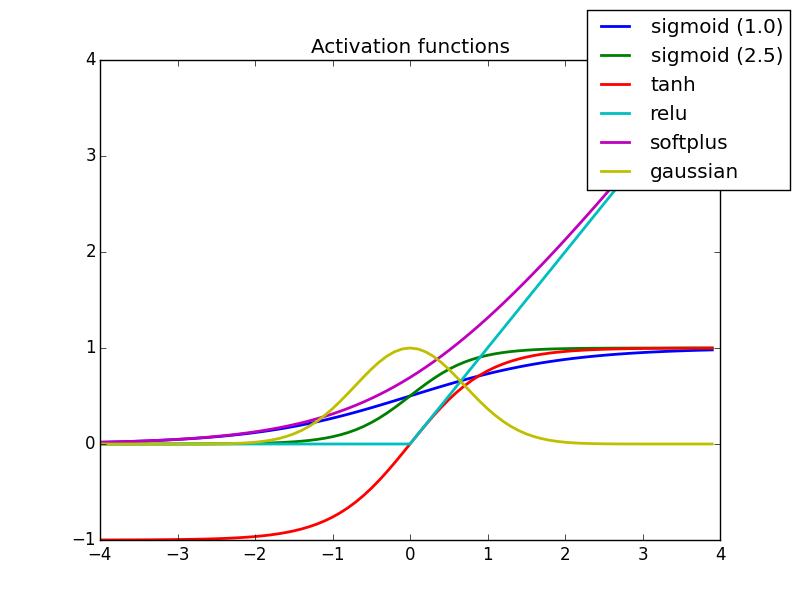
\includegraphics[width=0.8\linewidth,height=0.8\textheight,keepaspectratio]{results/activation_comparison/various_activation_functions.png}}
\caption{Comparison of activation function shapes (left) and their derivatives (right) for \(A_{\max} = 0.9487\) (16-QAM). Hardtanh has a sharp transition at the clip bounds; sigmoid and scaled tanh provide smooth saturation with non-zero gradients throughout.}\label{fig:fig36}
\end{figure}


\section{16-Class 2D Classification for QAM16}\label{sec:class-2d-classification-for-qam16}

\textbf{Goal:} Eliminate the structural BER floor imposed by per-axis I/Q splitting for 16-QAM by utilizing full 2D decision boundaries.

\textbf{Trials:} - \textbf{Topology:} SISO - \textbf{Modulation scheme:} 16-QAM - \textbf{Channel:} AWGN - \textbf{Equalizers:} None - \textbf{NN architecture:} Supervised (MLP, Hybrid), Generative (VAE, CGAN), Sequence (Transformer, Mamba S6, Mamba-2 SSD) - \textbf{NN activation:} None (Softmax implicitly via Cross-Entropy loss) - \textbf{Special case:} 16-class joint 2D classification

\textbf{Conclusion:} Treating the relay as a joint 16-point classifier over the full 2D constellation space completely eliminates the structural 4-class BER floor. For the first time, neural variants (VAE, Hybrid, Transformer, MLP) matched classical DF performance at high SNR, achieving near-zero BER at 20 dB; only the CGAN fails to converge in either formulation. This proves the previous BER floor was an artifact of I/Q splitting, not a fundamental limitation (Equation~\ref{eq:iq-splitting}) of neural relays.

\subsection{Results Tables}\label{sec:results-tables-5}

Table \ref{tbl:table24} \REV{Fix applied (data provenance): every cell of Table~\ref{tbl:table24} is now taken from the committed 16-class results file, and Figure~\ref{fig:fig51} was regenerated from that same file, both previously carried values from a superseded run, and the VAE and Hybrid cells were blank although the data existed. Table, figure, and captions now share one source. A former Table~16 (CSI/LayerNorm) and the three conclusions citing it were removed, since those experiments were cut in the restructure (Appendix~E).}
 presents the BER at 20 dB for all variants alongside the classical AF and DF baselines.

\begin{longtable}[]{@{}llll@{}}
\caption{BER at 20 dB for all relay variants: 4-class (I/Q split) vs.~16-class (joint 2D) classification for 16-QAM. Entries of 0.00000 correspond to zero errors observed within the trial budget (BER below the $\sim$$2\times10^{-4}$ resolution floor), so no finite improvement ratio is quoted for them.}\label{tbl:table24}\tabularnewline
\toprule\noalign{}
Relay & 4-cls BER @ 20 dB & 16-cls BER @ 20 dB & Improvement \\
\midrule\noalign{}
\endfirsthead
\toprule\noalign{}
Relay & 4-cls BER @ 20 dB & 16-cls BER @ 20 dB & Improvement \\
\midrule\noalign{}
\endhead
\bottomrule\noalign{}
\endlastfoot
MLP & 0.00867 & \textbf{0.00017} & 51x \\
VAE & 0.00867 & \textbf{0.00000} & --- \\
CGAN & 0.3530 & 0.2817 & --- \\
Hybrid & 0.00867 & \textbf{0.00000} & --- \\
trans-\\former & 0.00867 & \textbf{0.00000} & --- \\
Mamba S6 & 0.00867 & \textbf{0.00033} & 26x \\
Mamba2\\(ssd) & 0.00867 & \textbf{0.00167} & 5.2x \\
AF & 0.00083 &: &: \\
DF & 0.00000 &: &: \\
\end{longtable}

\subsection{Results Figures}\label{sec:results-figures-6}

\begin{figure}[H]
\centering
\centering
\pandocbounded{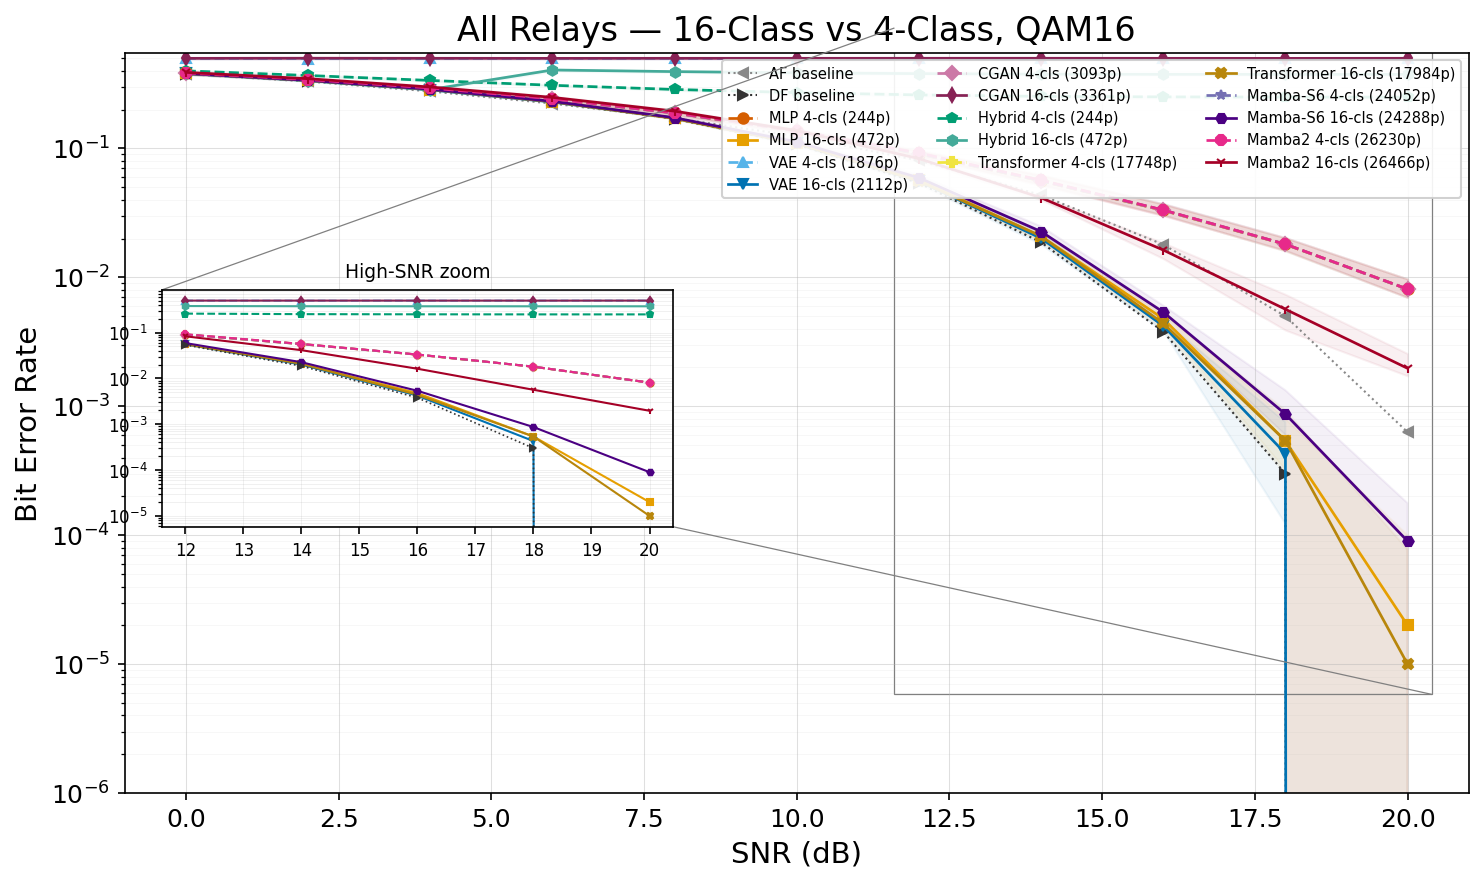
\includegraphics[width=\linewidth,height=\textheight,keepaspectratio]{results/all_relays_16class/ber_all_relays_16class.png}}
\caption{16-QAM BER vs.~SNR for all relay variants (4-class and 16-class) on AWGN. The 4-class variants (dashed) plateau at BER $\approx 0.008$ while the successfully trained 16-class variants (solid) continue decreasing, approaching and matching the DF baseline.}\label{fig:fig50}
\end{figure}

\begin{figure}[H]
\centering
\centering
\pandocbounded{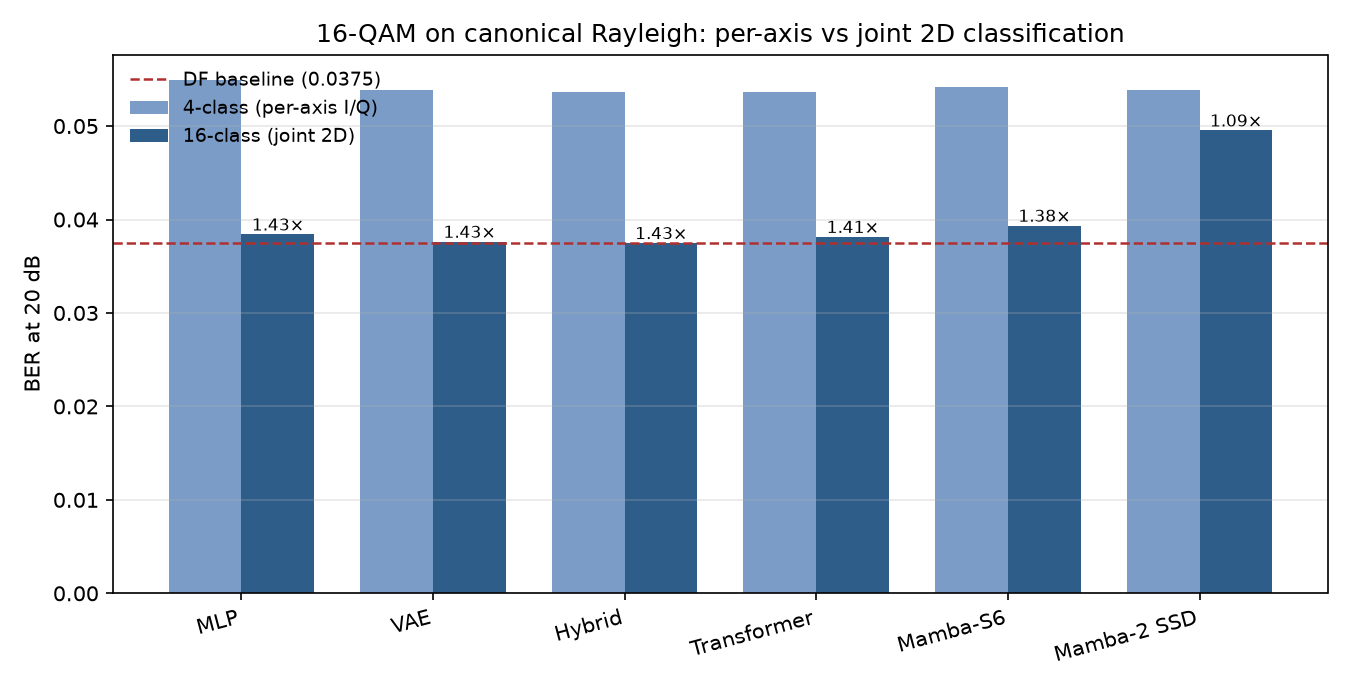
\includegraphics[width=\linewidth,height=\textheight,keepaspectratio]{results/all_relays_16class/grouped_bar_16class.png}}
\caption{Grouped bar comparison of 4-class vs.~16-class BER at 20 dB for each architecture. The joint 16-class formulation drives the BER to (near-)zero for every architecture except the CGAN, which fails to converge in both formulations (0.353 / 0.282) and dominates the plot at this scale.}\label{fig:fig51}
\end{figure}

\begin{figure}[H]
\centering
\centering
\pandocbounded{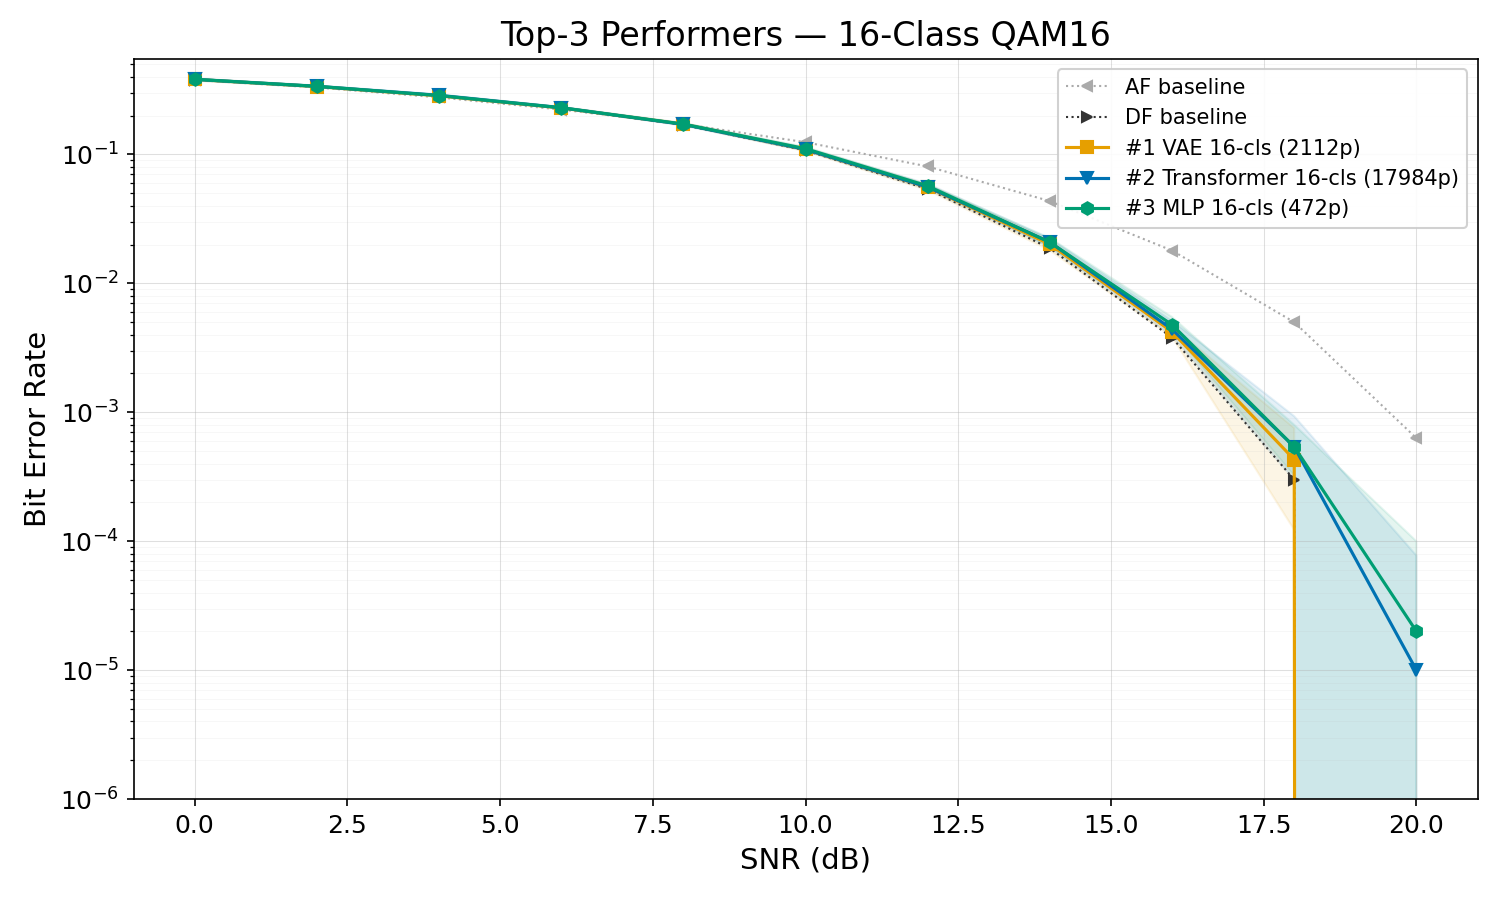
\includegraphics[width=\linewidth,height=\textheight,keepaspectratio]{results/all_relays_16class/top3_16class.png}}
\caption{Top-3 16-class relay variants compared against AF and DF. VAE 16-cls, Transformer 16-cls, and MLP 16-cls all match or approach DF performance across the full SNR range.}\label{fig:fig53}
\end{figure}
